\documentclass[table]{beamer}

\usepackage[spanish]{babel}
\usepackage[normalem]{ulem}
\usepackage{xcolor}
\usepackage{pgfgantt}
\usepackage{booktabs}
\usepackage{bookmark}
\usepackage{tabularx}
\usepackage{graphicx}
\usepackage{pgfplots}
\usepackage{multicol}
\usepackage{ragged2e}
\pgfplotsset{compat=newest}

\usepackage{tikz}
\usetikzlibrary{shapes.geometric, arrows.meta, fit, backgrounds, positioning, matrix, decorations.pathreplacing, calc}
\tikzstyle{startstop} = [rectangle, rounded corners, minimum width=3cm, minimum height=1cm,text centered, draw=black, fill=red!50]
\tikzstyle{io} = [trapezium, trapezium left angle=70, trapezium right angle=110, minimum width=3cm, minimum height=1cm, text centered, draw=black, fill=blue!30]
\tikzstyle{process} = [rectangle, minimum width=3cm, minimum height=1cm, text centered, draw=black, fill=orange!30]
\tikzstyle{decision} = [diamond, minimum width=3cm, minimum height=1cm, text centered, draw=black, fill=green!20]
\tikzstyle{database} = [cylinder, minimum width=3cm, minimum height=2cm, text centered, shape border rotate=90, aspect=0.25, draw=black, fill=yellow!30]
\tikzstyle{arrow} = [thick, ->, >=stealth]
\tikzstyle{line} = [-Latex]

\newcommand{\inline}[2]{%
    \begin{tikzpicture}[baseline=(word.base), txt/.style={shape=rectangle, inner sep=0pt}]
        \node[txt] (word) {\texttt{#1}};
        \node[above] at (word.north) {\footnotesize{#2}};
    \end{tikzpicture}%
}

\newlength\figureheight{}
\newlength\figurewidth{}
\setlength\figureheight{0.7\linewidth}
\setlength\figurewidth{\linewidth}

\apptocmd{\frame}{}{\justifying}{} % Allow optional arguments after frame.

\usetheme{metropolis}

\title{Estudio sobre Sistemas de Recomendación y Predicción basados en el procesamiento del lenguaje natural}
\date{\today}
\author{Hugo Ferrando Seage}
\institute{Universidad Europea de Madrid\\Escuela de Arquitectura, Ingeniería y Diseño}

\begin{document}
  \maketitle

  \section{Introducción}
  \begin{frame}[fragile]{Introducción}
      Los recomendadores son una parte esencial de cualquier servicio de Video on Demand y de otros sectores.

      \begin{multicols}{2}
          \begin{itemize}
              \item Netflix
              \item Movistar+
              \item Amazon
              \item Hulu
              \item HBO
              \item IMDb
              \item FilmAffinity
              \item Jinni
          \end{itemize}
      \end{multicols}
  \end{frame}

  \begin{frame}{Introducción}
      Existen tres grandes tipos de sistemas de recomendación:
      \begin{itemize}
          \item Filtrado colaborativo
          \item Filtrado por contenido
          \item Sistemas híbridos
      \end{itemize}
  \end{frame}

  \begin{frame}{Filtrado Colaborativo}
      Consiste en emparejar usuarios que tengan gustos similares y recomendar en base a esos datos.

      Los usuarios deben puntuar los contenidos, o se pueden usar otras métricas.

      Se puede visualizar usando una matriz donde las filas representan usuarios y la columnas representan productos.
  \end{frame}

  \begin{frame}{Filtrado por Contenido}
      Consiste en la creación de un modelo que determina la similitud entre productos en base a algún criterio.

      Ese criterio puede ser cualquier elemento del producto. Para películas puede ser el género. Para restaurantes el tipo de cocina. Etc.
  \end{frame}

  \begin{frame}{Filtrado Híbrido}
      Usan una combinación de ambas técnicas para complementar las recomendaciones.
  \end{frame}

  \section{Objetivos}

  \begin{frame}{Objetivos}
      \begin{itemize}
          \item Construir un recomendador de películas
          \item Crear el modelo en base a tres algoritmos
              \begin{itemize}
                  \item LSA
                  \item Doc2Vec
                  \item E-Modelo
              \end{itemize}
          \item Optimizar modelos
          \item Crear una interfaz desde donde poder probarlos
      \end{itemize}
  \end{frame}

  \section{Metodología}

  \begin{frame}{Metodología}
      La metodología usada ha sido ágil, basada en MVPs.

      \begin{figure}[!htbp]
          \resizebox{0.45\textwidth}{!}{
              \centering
              \begin{ganttchart}[
                  hgrid,
                  vgrid,
                  time slot format=isodate-yearmonth,
                  compress calendar
                  ]{2016-9}{2017-7} %chktex 8
                  \setganttlinklabel{f-s}{}

                  \gantttitlecalendar{year, month} \\
                  \ganttbar{Investigación}{2016-09}{2016-11} \\ %chktex 8
                  \ganttbar{Doc2Vec}{2017-03}{2017-03} \\ %chktex 8
                  \ganttbar{LSA MVP1}{2016-10}{2016-11} \\ %chktex 8
                  \ganttbar{LSA MVP2}{2016-12}{2017-01} \\ %chktex 8
                  \ganttbar{LSA MVP3}{2017-02}{2017-03} \\ %chktex 8
                  \ganttbar{ALS MVP1}{2016-09}{2016-12} \\ %chktex 8
                  \ganttbar{ALS MVP2}{2017-01}{2017-02} \\ %chktex 8
                  \ganttbar{ALS MVP3}{2017-03}{2017-03} \\ %chktex 8
                  \ganttbar{Desarrollo Interfaz}{2017-04}{2017-05} \\ %chktex 8
                  \ganttmilestone{Fin Desarrollo}{2017-05} \\ %chktex 8
                  \ganttbar{Documentación}{2017-05}{2017-06} \\ %chktex 8
                  \ganttmilestone{Entrega \& Presentación}{2017-06}{2017-06} %chktex 8

                  \ganttlink{elem0}{elem1}
                  \ganttlink{elem0}{elem2}

                  \ganttlink[link type=f-s]{elem2}{elem3}
                  \ganttlink[link type=f-s]{elem3}{elem4}

                  \ganttlink[link type=f-s]{elem5}{elem6}
                  \ganttlink[link type=f-s]{elem6}{elem7}

                  \ganttlink[link type=f-s]{elem1}{elem8}
                  \ganttlink[link type=f-s]{elem4}{elem8}
                  \ganttlink[link type=f-s]{elem7}{elem8}

                  \ganttlink{elem8}{elem9}
                  \ganttlink{elem10}{elem11}
              \end{ganttchart}
          }
      \end{figure}
  \end{frame}

  \section{Descarga de datos}

  \begin{frame}{Descarga de datos}
      \begin{figure}[!htbp]
          \resizebox{0.45\textwidth}{!}{
              \begin{tikzpicture}[node distance=2cm]
                  \centering
                  \node (init) [startstop] {Top 1000 IMDb};
                  \node (link1) [decision, below of=init] {URL};
                  \node (pelicula-init) [startstop, below of=link1] {Película};
                  \node (link2) [decision, below of=pelicula-init, yshift=-2cm] {URL};
                  \node (keywords) [process, right of=link2, xshift=2cm] {Palabras clave};
                  \node (info) [process, above of=keywords] {Información};
                  \node (reviews) [startstop, below of=link2] {Críticas};
                  \node (link3) [decision, below of=reviews] {URL};
                  \node (reviews-1) [process, right of=reviews, xshift=2cm] {Crítica};
                  \node (database) [database, right of=link1, xshift=3cm] {BD};
                  \begin{scope}[on background layer]
                      \node (bbox) [rectangle,draw,minimum width=2cm] [fit = (info) (keywords) (reviews-1),fill=yellow!30,label=above:Película] {};
                  \end{scope}

                  \draw [line] (init) -- (link1);
                  \draw [line] (link1) to [bend left] node[anchor=east] {página} (init);
                  \draw [line] (link1) -- node[anchor=north] {¿visitado?} (database);
                  \draw [line] (database) |- node[anchor=west] {no} (pelicula-init);
                  \draw [line] (pelicula-init) -- (link2);
                  \draw [line] (pelicula-init) |- (info);
                  \draw [line] (link2) -- (keywords);
                  \draw [line] (link2) -- (reviews);
                  \draw [line] (reviews) -- (link3);
                  \draw [line] (link3) to [bend left] node[anchor=east] {página} (reviews);
                  \draw [line] (link3) -| (reviews-1);
              \end{tikzpicture}
          }
      \end{figure}
  \end{frame}

  \section{Limpieza de textos}

  \begin{frame}[fragile]{Limpieza de textos}
      \begin{figure}
          \begin{verbatim}
              Zeus is a Greek God.
          \end{verbatim}
      \end{figure}

      \begin{figure}
          \inline{Zeus}{NNP} \inline{is}{VBZ} \inline{a}{DT} \inline{Greek}{NN} \inline{God}{NN}.
      \end{figure}
  \end{frame}

  \begin{frame}[fragile]{Limpieza de textos}
      \centering
      \begin{verbatim}
          Zeus is a country deity. (Hiperónimos)
      \end{verbatim}

      \begin{verbatim}
          is a country deity. (Nombres)
      \end{verbatim}

      \begin{verbatim}
          country deity (Stopwords)
      \end{verbatim}

      \begin{verbatim}
          counti deiti (Stemmer)
      \end{verbatim}
  \end{frame}

  \section{LSA}

  \begin{frame}{LSA}
      Latent Semantic Analysis trata de extraer conceptos de cada texto y analizar la relación entre documentos.
  \end{frame}

  \begin{frame}[fragile]{TF-IDF}
      \tiny
      \[tfidf =
          \begin{tikzpicture}[baseline=-0.65ex,scale=0.8]
              \matrix [matrix of math nodes,left delimiter=(,right delimiter=),row sep=0.5cm,column sep=0.5cm] (m) {
                  0.39&0.16&0.19&0.01&0.25&0.79&0.27 \\
                  0.12&0.12&0.06&0.46&0.21&0.07&0.83 \\
                  0.46&0.55&0.15&0.55&0.22&0.27&0.11 \\
                  0.00&0.60&0.51&0.00&0.00&0.60&0.00 \\
                  0.41&0.00&0.35&0.83&0.00&0.00&0.00 \\
              };
              \node[above=10pt of m-1-1, rotate=45, yshift=3mm, xshift=3mm] (top-1) {says};
              \node[above=10pt of m-1-2, rotate=45, yshift=3mm, xshift=3mm] (top-2) {just};
              \node[above=10pt of m-1-3, rotate=45, yshift=3mm, xshift=3mm] (top-3) {room};
              \node[above=10pt of m-1-4, rotate=45, yshift=3mm, xshift=3mm] (top-4) {dead};
              \node[above=10pt of m-1-5, rotate=45, yshift=3mm, xshift=3mm] (top-5) {asks};
              \node[above=10pt of m-1-6, rotate=45, yshift=3mm, xshift=3mm] (top-6) {ship};
              \node[above=10pt of m-1-7, rotate=45, yshift=3mm, xshift=3mm] (top-7) {mother};

              \node[left=12pt of m-1-1] (left-1) {The Matrix};
              \node[left=12pt of m-2-1] (left-2) {Alien};
              \node[left=12pt of m-3-1] (left-3) {Serenity};
              \node[left=12pt of m-4-1] (left-4) {Casablanca};
              \node[left=12pt of m-5-1] (left-5) {Amelie};
          \end{tikzpicture}
      \]
  \end{frame}

  \begin{frame}[fragile]{SVD}
      \tiny
      \[
          V^T =
          \begin{tikzpicture}[baseline=-0.65ex,scale=0.8]
              \matrix [matrix of math nodes,left delimiter=(,right delimiter=),row sep=0.5cm,column sep=0.5cm] (m) {
                  0.56&0.59&0.56&0.09&0.09 \\
                  0.12&-0.02&0.12&-0.69&-0.69 \\};

              \node[above=10pt of m-1-1, rotate=45, yshift=3mm, xshift=3mm] (top-1) {Matrix};
              \node[above=10pt of m-1-2, rotate=45, yshift=3mm, xshift=3mm] (top-2) {Alien};
              \node[above=10pt of m-1-3, rotate=45, yshift=3mm, xshift=3mm] (top-3) {Serenity};
              \node[above=10pt of m-1-4, rotate=45, yshift=3mm, xshift=3mm] (top-4) {Casablanca};
              \node[above=10pt of m-1-5, rotate=45, yshift=3mm, xshift=3mm] (top-5) {Amelie};

              \node[left=12pt of m-1-1] (left-1) {Sci-Fi topic};
              \node[left=12pt of m-2-1] (left-2) {Romance topic};

          \end{tikzpicture}
      \]
  \end{frame}

  \begin{frame}{Similitud Coseno}
      \begin{figure}[!htbp]
          \begin{equation}
              \cos\left(
                  \begin{tikzpicture}[baseline=-0.65ex,scale=0.8]
                      \matrix [matrix of math nodes,left delimiter=(,right delimiter=),row sep=0.5cm,column sep=0.5cm] (m) {0.56\\0.12\\};
                  \end{tikzpicture}
                  ,
                  \begin{tikzpicture}[baseline=-0.65ex,scale=0.8]
                      \matrix [matrix of math nodes,left delimiter=(,right delimiter=),row sep=0.5cm,column sep=0.5cm] (m) {0.59\\-0.02\\};
                  \end{tikzpicture}
              \right) = 0.97
          \end{equation}
          \caption{Alta similitud entre Matrix y Alien}
      \end{figure}

      \begin{figure}[!htbp]
          \begin{equation}
              \cos\left(
                  \begin{tikzpicture}[baseline=-0.65ex,scale=0.8]
                      \matrix [matrix of math nodes,left delimiter=(,right delimiter=),row sep=0.5cm,column sep=0.5cm] (m) {0.56\\0.12\\};
                  \end{tikzpicture}
                  ,
                  \begin{tikzpicture}[baseline=-0.65ex,scale=0.8]
                      \matrix [matrix of math nodes,left delimiter=(,right delimiter=),row sep=0.5cm,column sep=0.5cm] (m) {0.09\\-0.69\\};
                  \end{tikzpicture}
              \right) = -0.08
          \end{equation}
          \caption{Baja similitud entre Matrix y Amelie}
      \end{figure}
  \end{frame}

  \section{Doc2Vec}

  \begin{frame}{Word2Vec}
      Word2Vec es un algoritmo creado por Google en 2013. Es conceptualmente similar a LSA, pero teniendo en cuenta cada palabra dentro de su contexto.

      Es decir, calcula la probabilidad de que una palabra esté en la vecindad de otra palabra en el vocabulario.
  \end{frame}

  \begin{frame}{Word2Vec}
      \tiny
      \begin{table}
          \centering
          \begin{tabular}{cp{45mm}}
              \toprule
              Source Text & Training Samples \\
              \midrule
              \colorbox{blue!20}{\colorbox{red!20}{The} quick brown} fox jumps over the lazy dog & (`the', `quick') \newline (`the', `brown') \\
              \midrule
              \colorbox{blue!20}{The \colorbox{red!20}{quick} brown fox} jumps over the lazy dog & (`quick', `the') \newline (`quick', `brown') \newline (`quick', `fox') \\
              \midrule
              \colorbox{blue!20}{The quick \colorbox{red!20}{brown} fox jumps} over the lazy dog & (`brown', `the') \newline (`brown', `quick') \newline (`brown', `fox') \newline (`brown', `jumps') \\
              \midrule
              The \colorbox{blue!20}{quick brown \colorbox{red!20}{fox} jumps over} the lazy dog & (`fox', `quick') \newline (`fox', `brown') \newline (`fox', `jumps') \newline (`fox', `over') \\
              \bottomrule
          \end{tabular}
      \end{table}
  \end{frame}

  \begin{frame}{Word2Vec}
      \begin{table}
          \centering
          \begin{tabular}{ccc}
              \toprule
              Palabra & Posición por orden alfabético & Vector\\
              \midrule
              fox & 2/3 & [0, 1, 0]\\
              dog & 1/3 & [1, 0, 0]\\
              zebra & 3/3 & [0, 0, 1]\\
              \bottomrule
          \end{tabular}
      \end{table}
  \end{frame}

  \begin{frame}{Word2Vec}
      \centering
      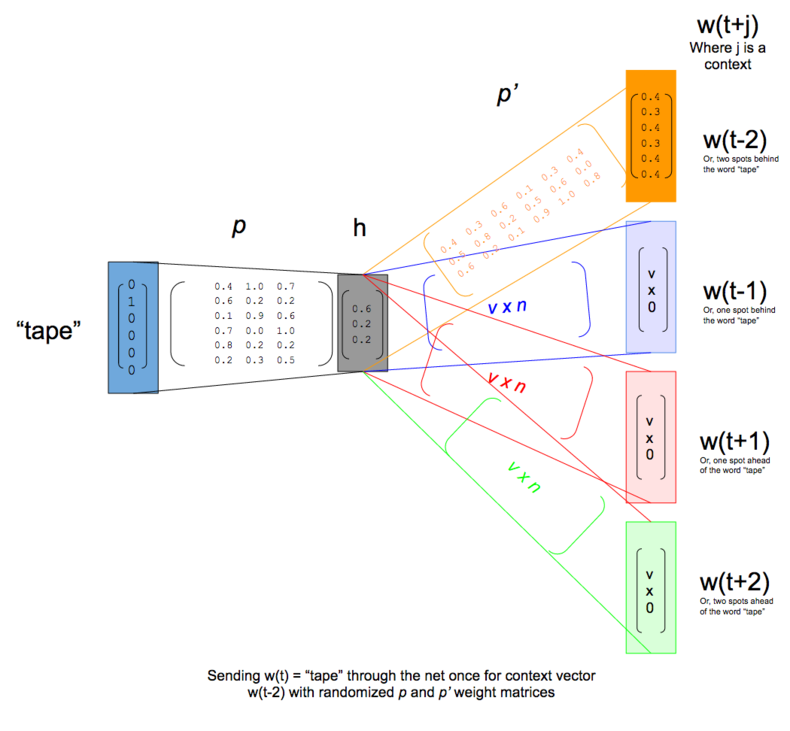
\includegraphics[scale=0.65]{./figures/skip-gram-exp.png}
  \end{frame}

  \section{E-Modelo}

  \begin{frame}{E-Modelo}
      Modelo de predicción de frecuencia de uso de palabras híbrido.

      Combina el filtrado colaborativo con los features extraidos de un filtrado por contenido.
  \end{frame}

  \begin{frame}[fragile]{E-Modelo}
      \small
      \centering
      \begin{tikzpicture}[every node/.style={anchor=north east,fill=white,minimum width=1cm,minimum height=5mm}]
          \matrix (mA) [draw,matrix of math nodes]
          {
              1 & 1 & 0 \\
              0 & 1 & 0 \\
              -1 & -1 & -1 \\
          };

          \matrix (mB) [draw,matrix of math nodes] at ($(mA.south west)+(1.5,0.7)$)
          {
              -1 & -1 & -1 \\
              0 & 2 & 0 \\
              -1 & -1 & -1 \\
          };

          \matrix (mC) [draw,matrix of math nodes] at ($(mB.south west)+(1.5,0.7)$)
          {
              -1 & -1 & -1 \\
              0 & 1 & 0 \\
              0 & 0 & 2 \\
          };

          \node[above=10pt of mA-1-1, rotate=45, yshift=1mm, xshift=8mm] (top-1) {Palabra 1};
          \node[above=10pt of mA-1-2, rotate=45, yshift=1mm, xshift=8mm] (top-2) {Palabra 2};
          \node[above=10pt of mA-1-3, rotate=45, yshift=1mm, xshift=8mm] (top-3) {Palabra 3};

          \node[left=12pt of mC-1-1] (left-1) {Usuario 1};
          \node[left=12pt of mC-2-1] (left-2) {Usuario 2};
          \node[left=12pt of mC-3-1] (left-3) {Usuario 3};

          \node[right=12pt of mC-2-3, yshift=-3mm] (right-1) {Producto 3};
          \node[right=12pt of mB-2-3, yshift=-3mm] (right-2) {Producto 2};
          \node[right=12pt of mA-2-3, yshift=-3mm] (right-3) {Producto 1};

          \draw[dashed](mA.north east)--(mC.north east);
          \draw[dashed](mA.north west)--(mC.north west);
          \draw[dashed](mA.south east)--(mC.south east);
      \end{tikzpicture}
  \end{frame}

  \begin{frame}[fragile]{E-Modelo}
      \centering
      \tiny
      \begin{tikzpicture}[baseline=-0.65ex,scale=0.8,decoration=brace]
          \matrix [matrix of math nodes,left delimiter=(,right delimiter=),row sep=0.5cm,column sep=0.5cm] (m)
          {
              1 & 1 & 0 & -1 & -1 & -1 & -1 & -1 & -1 \\
              0 & 1 & 0 & 0 & 2 & 0 & 0 & 1 & 0 \\
              -1 & -1 & -1 & -1 & -1 & -1 & 0 & 0 & 2 \\
          };
          \node[above=10pt of m-1-1, rotate=45, yshift=3mm, xshift=3mm] (top-1) {Palabra 1};
          \node[above=10pt of m-1-2, rotate=45, yshift=3mm, xshift=3mm] (top-2) {Palabra 2};
          \node[above=10pt of m-1-3, rotate=45, yshift=3mm, xshift=3mm] (top-3) {Palabra 3};
          \node[above=10pt of m-1-4, rotate=45, yshift=3mm, xshift=3mm] (top-4) {Palabra 1};
          \node[above=10pt of m-1-5, rotate=45, yshift=3mm, xshift=3mm] (top-5) {Palabra 2};
          \node[above=10pt of m-1-6, rotate=45, yshift=3mm, xshift=3mm] (top-6) {Palabra 3};
          \node[above=10pt of m-1-7, rotate=45, yshift=3mm, xshift=3mm] (top-7) {Palabra 1};
          \node[above=10pt of m-1-8, rotate=45, yshift=3mm, xshift=3mm] (top-8) {Palabra 2};
          \node[above=10pt of m-1-9, rotate=45, yshift=3mm, xshift=3mm] (top-9) {Palabra 3};

          \node[left=20pt of m-1-1] (left-1) {Usuario 1};
          \node[left=20pt of m-2-1] (left-2) {Usuario 2};
          \node[left=15pt of m-3-1] (left-3) {Usuario 3}; % why not aligned?

          \draw[decorate,transform canvas={yshift=2cm},thick] (m-1-1.north west) -- node[above=2pt] {Producto 1} (m-1-3.north east);
          \draw[decorate,transform canvas={yshift=2cm},thick] (m-1-4.north west) -- node[above=2pt] {Producto 2} (m-1-6.north east);
          \draw[decorate,transform canvas={yshift=2cm},thick] (m-1-7.north west) -- node[above=2pt] {Producto 3} (m-1-9.north east);
      \end{tikzpicture}

      40\% de precisión

  \end{frame}

  \section{Optimización}

  \begin{frame}{Parámetros LSA}
      \begin{itemize}
          \item Número de `features' TF-IDF
          \item Número de componentes LSA
          \item Frecuencia Mínima de Documentos
          \item Frecuencia Máxima de Documentos
      \end{itemize}
  \end{frame}

  \begin{frame}{Parámetros Doc2Vec}
      \begin{itemize}
          \item Size
          \item Window
          \item Minimum Word Count
          \item Iteraciones
      \end{itemize}
  \end{frame}

  \begin{frame}{Optimización LSA 2001: A Space Odyssey}
      \tiny
      \centering
      % This file was created by matplotlib2tikz v0.6.11.
\begin{tikzpicture}

\definecolor{color0}{rgb}{0.483870967741935,1,0.483870967741936}

\begin{axis}[
xlabel={Películas},
ylabel={Posición de la recomendación},
xmin=-0.433685551148337, xmax=6.3448234626804,
ymin=0, ymax=58.081737012987,
width=\figurewidth,
height=\figureheight,
xtick={0,1,2,3,4,5,6},
xticklabels={Gravity,Solaris,Interstellar,Alien,The Martian,Planet of.,Distrito 9},
tick align=outside,
xticklabel style = {rotate=45},
tick pos=left,
x grid style={lightgray!92.026143790849673!black},
y grid style={lightgray!92.026143790849673!black},
legend entries={{feat 2000 cmpn 1000 mndf 5 mxdf 100 keyw 0\% lsa 100\% tot 137},{feat 5000 cmpn 1000 mndf 5 mxdf 100 keyw 0\% lsa 100\% tot 117},{feat None cmpn 1000 mndf 5 mxdf 100 keyw 0\% lsa 100\% tot 96}},
legend style={at={(0.03,0.97)}, anchor=north west, draw=white!80.0!black},
legend cell align={left}
]
\addplot [only marks, draw=blue!50.0!black, fill=blue!50.0!black, colormap/viridis]
table{%
x                      y
-5.420625617958866e-03 +1.000000000000000e+00
+1.086622088194287e+00 +5.000000000000000e+00
+1.995440067901144e+00 +7.000000000000000e+00
+3.078365322052515e+00 +1.300000000000000e+01
+4.043780263625694e+00 +1.400000000000000e+01
+4.946125615546470e+00 +4.200000000000000e+01
+5.977704951936783e+00 +5.500000000000000e+01
};
\addplot [only marks, draw=color0, fill=color0, colormap/viridis]
table{%
x                      y
-8.528152414794855e-02 +1.000000000000000e+00
+9.718706170388742e-01 +4.000000000000000e+00
+2.107066229334886e+00 +1.000000000000000e+01
+2.922658544319798e+00 +1.100000000000000e+01
+4.069389572958468e+00 +1.300000000000000e+01
+5.083171633766593e+00 +2.700000000000000e+01
+5.979475177772462e+00 +5.100000000000000e+01
};
\addplot [only marks, draw=red!50.0!black, fill=red!50.0!black, colormap/viridis]
table{%
x                      y
-4.725123114241665e-02 +1.000000000000000e+00
+9.359426374888414e-01 +4.000000000000000e+00
+2.052841684428433e+00 +9.000000000000000e+00
+3.055576540820828e+00 +1.000000000000000e+01
+3.924672303573277e+00 +1.300000000000000e+01
+5.152248526925555e+00 +2.100000000000000e+01
+5.995823104116642e+00 +3.800000000000000e+01
};
\addplot [semithick, blue!50.0!black, opacity=0.5, forget plot]
table {%
0 -6.46428571428571
1 2.21428571428572
2 10.8928571428572
3 19.5714285714286
4 28.25
5 36.9285714285714
6 45.6071428571429
};
\addplot [semithick, color0, opacity=0.5, forget plot]
table {%
0 -4.60714285714285
1 2.50000000000001
2 9.60714285714286
3 16.7142857142857
4 23.8214285714286
5 30.9285714285714
6 38.0357142857143
};
\addplot [semithick, red!50.0!black, opacity=0.5, forget plot]
table {%
0 -2.25
1 3.07142857142857
2 8.39285714285714
3 13.7142857142857
4 19.0357142857143
5 24.3571428571429
6 29.6785714285714
};
\end{axis}

\end{tikzpicture}
  \end{frame}

  \begin{frame}{Optimización Doc2Vec 2001: A Space Odyssey}
      \tiny
      \centering
      % This file was created by matplotlib2tikz v0.6.11.
\begin{tikzpicture}

\definecolor{color0}{rgb}{0,0.833333333333333,1}
\definecolor{color1}{rgb}{1,0.901234567901234,0}

\begin{axis}[
xlabel={Películas},
ylabel={Posición de la recomendación},
xmin=-0.407733023228943, xmax=6.46414904806693,
ymin=0, ymax=81.8391458882914,
width=\figurewidth,
height=\figureheight,
xtick={0,1,2,3,4,5,6},
xticklabels={Solaris,Interstellar,Distrito 9,Planet of the.,Alien,Gravity,The Martian},
tick align=outside,
xticklabel style = {rotate=45},
tick pos=left,
x grid style={lightgray!92.026143790849673!black},
y grid style={lightgray!92.026143790849673!black},
legend cell align={left},
legend style={at={(0.03,0.97)}, anchor=north west, draw=white!80.0!black},
legend entries={{size 1000 window 3 minc 5 iter 10 tot 129},{size 1000 window 5 minc 5 iter 10 tot 111},{size 1000 window 8 minc 5 iter 10 tot 143},{size 1000 window 10 minc 5 iter 10 tot 163}}
]
\addplot [only marks, draw=blue!50.0!black, fill=blue!50.0!black, colormap/viridis]
table{%
x                      y
+3.506846797043030e-02 +0.000000000000000e+00
+9.817581206778054e-01 +9.000000000000000e+00
+1.900039319227744e+00 +1.600000000000000e+01
+2.972896629068051e+00 +1.100000000000000e+01
+4.014181472363457e+00 +8.000000000000000e+00
+4.950734114600046e+00 +2.600000000000000e+01
+6.053107328800729e+00 +5.900000000000000e+01
};
\addplot [only marks, draw=color0, fill=color0, colormap/viridis]
table{%
x                      y
+1.358059926847923e-03 +0.000000000000000e+00
+9.665157776728900e-01 +1.100000000000000e+01
+1.938385264546487e+00 +1.600000000000000e+01
+2.997964059782109e+00 +1.000000000000000e+01
+4.085108167334652e+00 +1.700000000000000e+01
+5.044467882064920e+00 +2.100000000000000e+01
+6.034366658357040e+00 +3.600000000000000e+01
};
\addplot [only marks, draw=color1, fill=color1, colormap/viridis]
table{%
x                      y
+5.723640351712631e-02 +0.000000000000000e+00
+1.065848370403365e+00 +7.000000000000000e+00
+1.956608785440840e+00 +1.000000000000000e+01
+2.934118262926154e+00 +2.000000000000000e+01
+3.972813047696823e+00 +2.200000000000000e+01
+5.124773606719176e+00 +1.400000000000000e+01
+6.089952328607143e+00 +7.000000000000000e+01
};
\addplot [only marks, draw=red!50.0!black, fill=red!50.0!black, colormap/viridis]
table{%
x                      y
-5.432506763021979e-02 +0.000000000000000e+00
+9.834196511509600e-01 +9.000000000000000e+00
+2.088062171591054e+00 +1.300000000000000e+01
+3.010015936142026e+00 +2.000000000000000e+01
+4.077112939890906e+00 +1.800000000000000e+01
+5.026803720925459e+00 +2.600000000000000e+01
+6.110741092468205e+00 +7.700000000000000e+01
};
\addplot [semithick, blue!50.0!black, opacity=0.5, forget plot]
table {%
0 -3.32142857142857
1 3.92857142857143
2 11.1785714285714
3 18.4285714285714
4 25.6785714285714
5 32.9285714285714
6 40.1785714285714
};
\addplot [semithick, color0, opacity=0.5, forget plot]
table {%
0 2.03571428571429
1 6.64285714285714
2 11.25
3 15.8571428571429
4 20.4642857142857
5 25.0714285714286
6 29.6785714285714
};
\addplot [semithick, color1, opacity=0.5, forget plot]
table {%
0 -4.85714285714285
1 3.57142857142858
2 12
3 20.4285714285714
4 28.8571428571429
5 37.2857142857143
6 45.7142857142857
};
\addplot [semithick, red!50.0!black, opacity=0.5, forget plot]
table {%
0 -5.64285714285714
1 4.00000000000001
2 13.6428571428571
3 23.2857142857143
4 32.9285714285714
5 42.5714285714286
6 52.2142857142857
};
\end{axis}

\end{tikzpicture}
  \end{frame}

  \section{Demo}

  \begin{frame}{Demo}
      \url{https://moviepepper.hugofs.com}
  \end{frame}
\end{document}
